\chapter[Opis projektu]{Opis projektu}

\section[Treść zadania]{Treść zadania}

\par{Zaprojektować i zaimplementować usługę udostępniania danych statystycznych na temat studentów uczelni wyższej, przy założeniu bezpiecznej i niezawodnej dystrybucji danych wrażliwych - poufnych informacji o studentach.}

\par{Usługa powinna:}
\begin{itemize}


\item mieć dokładnie jeden ten sam tekstowy plik konfiguracyjny dla części 
serwerowej i klientów usługi,
\item składać się po stronie serwerowej z dwóch warstw: (1)  wewnętrznej
  wytwarzającej, przechowującej i przesyłającej przetworzoną wrażliwą
informację, (2) warstwy zewnętrznej do udostępniania przetworzonej informacji
oprogramowaniu klienckiemu usługi,
\item oprogramowanie realizujące część serwerową powinno być współbieżne,
\item składać się po stronie klienckiej z prostych narzędzi opatulających
  zaproponowane API protokołu komunikacyjnego,
\item zapewniać odporność na uszkodzenia węzła, stąd każda z warstw powinna być
  uruchomiona na co najmniej dwóch węzłach,
\item zapewniać realizację usługi w trakcie awarii w czasie obsługi,
\item obsługiwać scenariusz próby ponownego wpięcia się przez węzeł dowolnej z
  warstw, z którym wcześniej utracono łączność, a zarazem być odporną na próbę
zastąpienia nieosiągalnego sieciowo węzła (np. w wyniku ataku DoS, odmowa
usługi) węzłem wrogim do tego nieuprawnionym,
\item na bieżąco i transparentnie dla oprogramowania klienckiego zarządzać
  dostępnymi zasobami lokalizacyjnymi,
\item zapewniać zadany (większy niż 1 ale dopuszczalny konfiguracją mniejszy niż
  liczba serwerów danych) poziom redundancji - z obsługą uzupełniania kopii na
innych serwerach w przypadku awarii włącznie,
\item cała część sewerowa usługi powinna być uruchamiana i zamykana jednokrotnym
  wywołaniem skryptu na jednym węźle serwera z jednym argumentem
<start|stop|status> (wykorzystanie nieinteraktywnych metod automatycznego
uwierzytelniania węzłów w SSH).

\end{itemize}

\section[Opis rozwiązania]{Opis rozwiazania}

\par{Nasze rowiązanie to rozproszony system do rejestracji studentów uczelnii wyższych na przemioty. Warstwą wewnątrzną przechowujące dane wrażliwe, w tym przypadku będą węzły rejestrujące studentów ideowo umieszczone w dziekanatach instytutów i obsługiwane przez osoby tam pracujące. Warstwa pośrednia przechowuje informacje o studentach, jednak bez informacji wrażliwej, wie tylko, że istnieje student zapisany na przedmioty RSO, SOI, ANA1 i RS,  nie wie więc, że  student ten nazywa się Jak Kowalski. Owe dane są przetwarzane na żadanie aplikacji klienckiej, dostępnej dla studentów, którzy chcą dowiedzieć się, ile osób zapisanych jest na dany przedmiot.}

\section[Wstępny projekt architektury]{Wstępny projekt architektury}

\par{Wewnętrzna warstwa serwera wytwarza i przechowuje informacje na temat studentów uczelni wyższej - stworzone na podstawie danych wprowadzonych przez pracowników dziekanatu. Następnie ów warstwa przesyła informacje do warstwy zewnętrznej serwera (warstwy przetwarzającej) świadczącej usługi udostępniania informacji przetworzonej rozwiązaniom klienckim. Każda z warst komunikować się będzie z użyciem protokołu TCP/IP przesyłając wiadomości zserializowane za pomocą Google Protocols Buffer.}

\begin{figure}[h]
\begin{center}
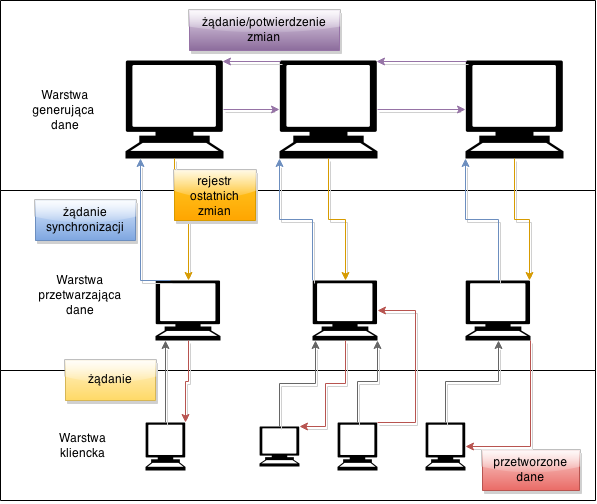
\includegraphics[width=0.9\linewidth]{img/dane_net.png} 
\caption{Diagram ilustrujący komunikację pomiędzy poszczególnymi warstwami}
\label{img:docker_tut1}
\end{center}
\end{figure}

\subsection*[Warstwa wewnętrzna serwera]{Warstwa wewnętrzna serwera}

\par{Warstwa stworzona w technologii token ring. Węzły połączone są w pierścień i przesyłają sobie kolejno token zawierający informacje o potencjalnych zmianach. Tylko węzeł posiadający token może wykonywać operację aktualizacji danych. Każda zmiana musi być zatwierdzona przez pozostałe węzły. Zapewnia to synchronizację danych oraz bieżące sprawdzenie działania pozostałych węzłów. Szczegółowe informacje na ten temat znajdują się w podrozdziale \ref{z:sw}.}

\par{Dane wrażliwe przechowywane są w postaci rekordów zawierających:}

\begin{itemize}
\item ID studenta
\item imię studenta
\item nazwisko studenta
\item datę urodzenia
\item listę przedmiotów na jakie jest zapisany
\end{itemize}

\par{}

\subsection*[Warstwa zewnętrzna serwera]{Warstwa zewnętrzna serwera (warstwa przetwarzająca)}

\par{Warstwa przeznaczona do komunikacji z aplikacją kliencką. Na żadanie klienta przetwarza wcześniej otrzymane od warstwy wewnętrznej dane i wynik przetwarzania zwraca klientowi. Moduł ten synchronizuje dane, co zadany przez plik konfiguracyjny czas, tak aby administrator sam był wstanie dostosować interwał do aktualnych potrzeb. }

\begin{itemize}
\item ID studenta
\item listę przedmiotów na jakie jest zapisany
\end{itemize}

\subsection*[Aplikacja kliencka]{Aplikacja kliencka}

\par{Warstwa przeznaczona dla klienta to z założenia lekka i  intuicyjna aplikacja konsolowa. Moduł ten bezpośrednio łączyć będzie się tylko z modułem zewnętrznym serwera. Użytkownik, za pomocą tej aplikacji będzie mógł dowiedzieć się ile osób w danym momencie jest zapisany na wybranie przez niego przedmiot.}

\section[Opis szczegółowy]{Opis szczegółowy}

\subsection[Założenia]{Założenia}



\subsubsection*[Założenia ogólne]{Założenia ogólne} \label{z:o}

\begin{center}

\begin{tabular}{|c|c|l|l|}
\hline
\textbf{ID} & \textbf{Założenie} & \textbf{Szczegóły} & \textbf{Powody decyzji} \\
\hline
\label{z:o1} O1 & 
Protokół TCP/IP & 
Komunikacja między warstwami (wewnętrzna serwera - zewnętrzna serwera jak i zewnętrzna serwera - klienci) odbywa się za pomocą protokołów TCP/IP, wykorzystując Google Protocol Buffer (więcej w podrozdziale \ref{protobuf}).
& Protokół został przez nas wybrany ze względu na elastyczność dla różnych konfiguracji serwerów, tzn. bez względu na to czy warstwy serwera będą działały w obrębie jednego węzła czy nie protokół pozwoli na poprawną komunikację. W przypadku działania obu warstw serwera na jednym komputerze czy nawet w jednym procesie wydajność będzie mniejsza (w porównaniu np. do pamięci współdzielonej), jednak ze względu na ograniczony czas projektu i mniejsze skomplikowanie zostało wybrane to rozwiązanie. \\
\hline
\label{z:o2} O2 & Plik konfiguracyjny & 
 Każdy z węzłów danej warstwy będzie posiadała plik konfiguracyjny o tej samej strukturze. W zależności od typu dane z pliku zostaną odpowiednio skonfigurowane. Plik będzie zawierał: ID węzła, listę serwerów (zależnie od typu zewnętrznych lub wewnętrznych), dodatkowe dane konfiguracyjne (np. odpowiadających za redundancję danych, okresową synchronizację, itd.) &
Takie rozwiązanie jest wymagane w treści zadania. Ponadto ujednolica i ułatwia konfigurację projektu bez potrzeby ponownej kompilacji.\\
\hline
\label{z:o3} O3 & Proste komendy serwera &  
Warstwy serwera będą uruchamiane i zamykane jednokrotnym wywołaniem skryptu na danym węźle serwera z jednym argumentem: start, stop oraz status, które będą kolejno: uruchamiać usługi serwera, wyłączać usługi serwera oraz wyświetlać status serwera. & 
Takie rozwiązanie jest wymagane w treści zadania. Ponadto pozwoli na łatwą obsługę i testowanie części serwerowej systemu. \\
\hline

\end{tabular} 

\subsubsection*[Założenia dotyczące warstwy wewnętrznej serwera]{Założenia dotyczące warstwy wewnętrznej serwera} \label{z:sw}

\begin{tabular}{|c|c|l|l|}
\hline
\textbf{ID} & \textbf{Założenie} & \textbf{Szczegóły} & \textbf{Powody decyzji} \\
\hline
\label{z:sw1} SW1 & Technologia token ring &  - & - \\
\hline
\label{z:sw2} SW2 & Zmiana jednego rekordu na raz &  - & - \\
\hline
\label{z:sw3} SW3 & Bazy danych MySQL & Aplikacja serwerowa wewnętrzna będzie działać w oparciu o relacyjną bazę danych MySQL & 
Baza MySQL jest popularnym systemem relacyjnych baz danych z dobrą dokumentacją oraz szeroką i aktywną społecznością użytkowników. Ponadto system ten jest powszechnie znany wśród wszystkich członków projektu. Dodatkowo MySQL dobrze współpracuje z wybranym językiem programowania Java.
\\
\hline
\label{z:sw4} SW4 & - &  - & - \\
\hline
\label{z:sw5} SW5 & - &  - & - \\
\hline
\label{z:sw6} SW6 & - &  - & - \\
\hline
\label{z:sw7} SW7 & - &  - & - \\
\hline

\end{tabular} 

\subsubsection*[Założenia dotyczące warstwy zewnętrznej serwera]{Założenia dotyczące warstwy zewnętrznej serwera} \label{z:sz}

\begin{tabular}{|c|c|l|l|}
\hline
\textbf{ID} & \textbf{Założenie} & \textbf{Szczegóły} & \textbf{Powody decyzji} \\
\hline
\label{z:sz1} SZ1 & Wysyłanie ,,heartbeatów'' &  Zewnętrzne warstwy & - \\
\hline
\label{z:sz2} SZ2 & Okresowa synchronizacja &  - & - \\
\hline
\label{z:sz3} SZ3 & Redundacja danych &  - & - \\
\hline
\label{z:sz4} SZ4 & Udostępnianie usług &  - & - \\
\hline
\label{z:sz5} SZ5 & Obliczanie danych statystycznych &  - & - \\
\hline
\label{z:sz6} SZ6 & Lista serwerów &  - & - \\
\hline
\end{tabular} 

\subsubsection*[Założenia dotyczące aplikacji klienckiej]{Założenia dotyczące aplikacji klienckiej} \label{z:k}

\begin{tabular}{|c|c|l|l|}
\hline
\textbf{ID} & \textbf{Założenie} & \textbf{Szczegóły} & \textbf{Powody decyzji} \\
\hline
\label{z:k1} K1 & Brak logowania i autoryzacji użytkownika &  - & - \\
\hline
\label{z:k2} K2 & Brak interfejsu graficznego &  - & - \\
\hline
\label{z:k3} K3 & Usługa wyliczania danych statystycznych &  - & - \\
\hline
\label{z:k4} K4 & Lista serwerów &  - & - \\
\hline
\end{tabular} 

\end{center}

\subsection[Wymagania funkcjonalne]{Wymagania funkcjonalne}

\subsection[Wymagania niefunkcjonalne]{Wymagania niefunkcjonalne}

\section[Potencjalne problemy]{Potencjalne problemy}

\section[Organizacja środowiska programistycznego]{Organizacja środowiska programistycznego}